\clearpage

\chapter{Klassendiagramm}
Das Klassendiagramm enthält die folgenden Klassen:\\

\noindent \textbf{Main: } Start des Programms, Daten werden von Festplatte geladen \\ \\
\textbf{Menue: } Hauptmenue wird geladen, Eingabedaten des Benutzers entgegengenommen, die Klassen InputData, GameLayout, GameField und GameController werden erstellt \\ \\
\textbf{Card: } Stellt die Funktionen der Memorykarte zur Verfügung, informiert GameController bei Auswahl einer Karte \\ \\
\textbf{GameField: } erstellt das Spielfeld, mischt Karten\\ \\
\textbf{GameLayout: } liefert das Layout für das Spielfeld, wird von Player und GameController über Änderungen benachrichtigt, um geänderte Daten (z.B. Punkte) auf der GUI anzuzeigen\\ \\
\textbf{GridBagLayoutModel: }Hilfsklasse für GameLayout\\ \\
\textbf{InputData: } Datenspeicher für Spieler und Spielmodus\\ \\
\textbf{Player: } repräsentiert den Spieler und seine Daten, enthält Funktion um Punkte hinzuzufügen\\ \\
\textbf{Playerpool: } Verwaltet alle gespeicherten Spieler\\ \\
\textbf{GameController: } Steuert den Spielablauf\\ \\
\textbf{SaveObject: } Nimmt Playerpool und Highscore auf um sie gekapselt zu speichern\\ \\
\textbf{Highscore: } Verwaltet HighscoreData-Objekte, stellt sortierte Liste der 10 Besten Spieler bereit\\ \\
\textbf{HighscoreData: } Enthält Spieler und die erreichten Punkte pro gespieltem Spiel \\ \\
\textbf{HddSave: } Stellt Funktionen zum Speichern und Laden des SaveObjects bereit\\ \\
\textbf{WindowModel: } Vorlage für ein modifiziertes JFrame, wird von der Klasse Menue und GameLayout genutzt \\ \\

\textbf{Bemerkung: }Für die Klassen Menue, GameLayout und GameController sind im Klassendiagramm aufgrund der Übersichtlichkeit und Platzmangels nicht alle Membervariablen abgebildet. Deshalb sind diese zusätzlich mit vollständigen Membervariablen nach dem Klassendiagramm aufgeführt.
    
 
\begin{figure}[!h]
	\centering
    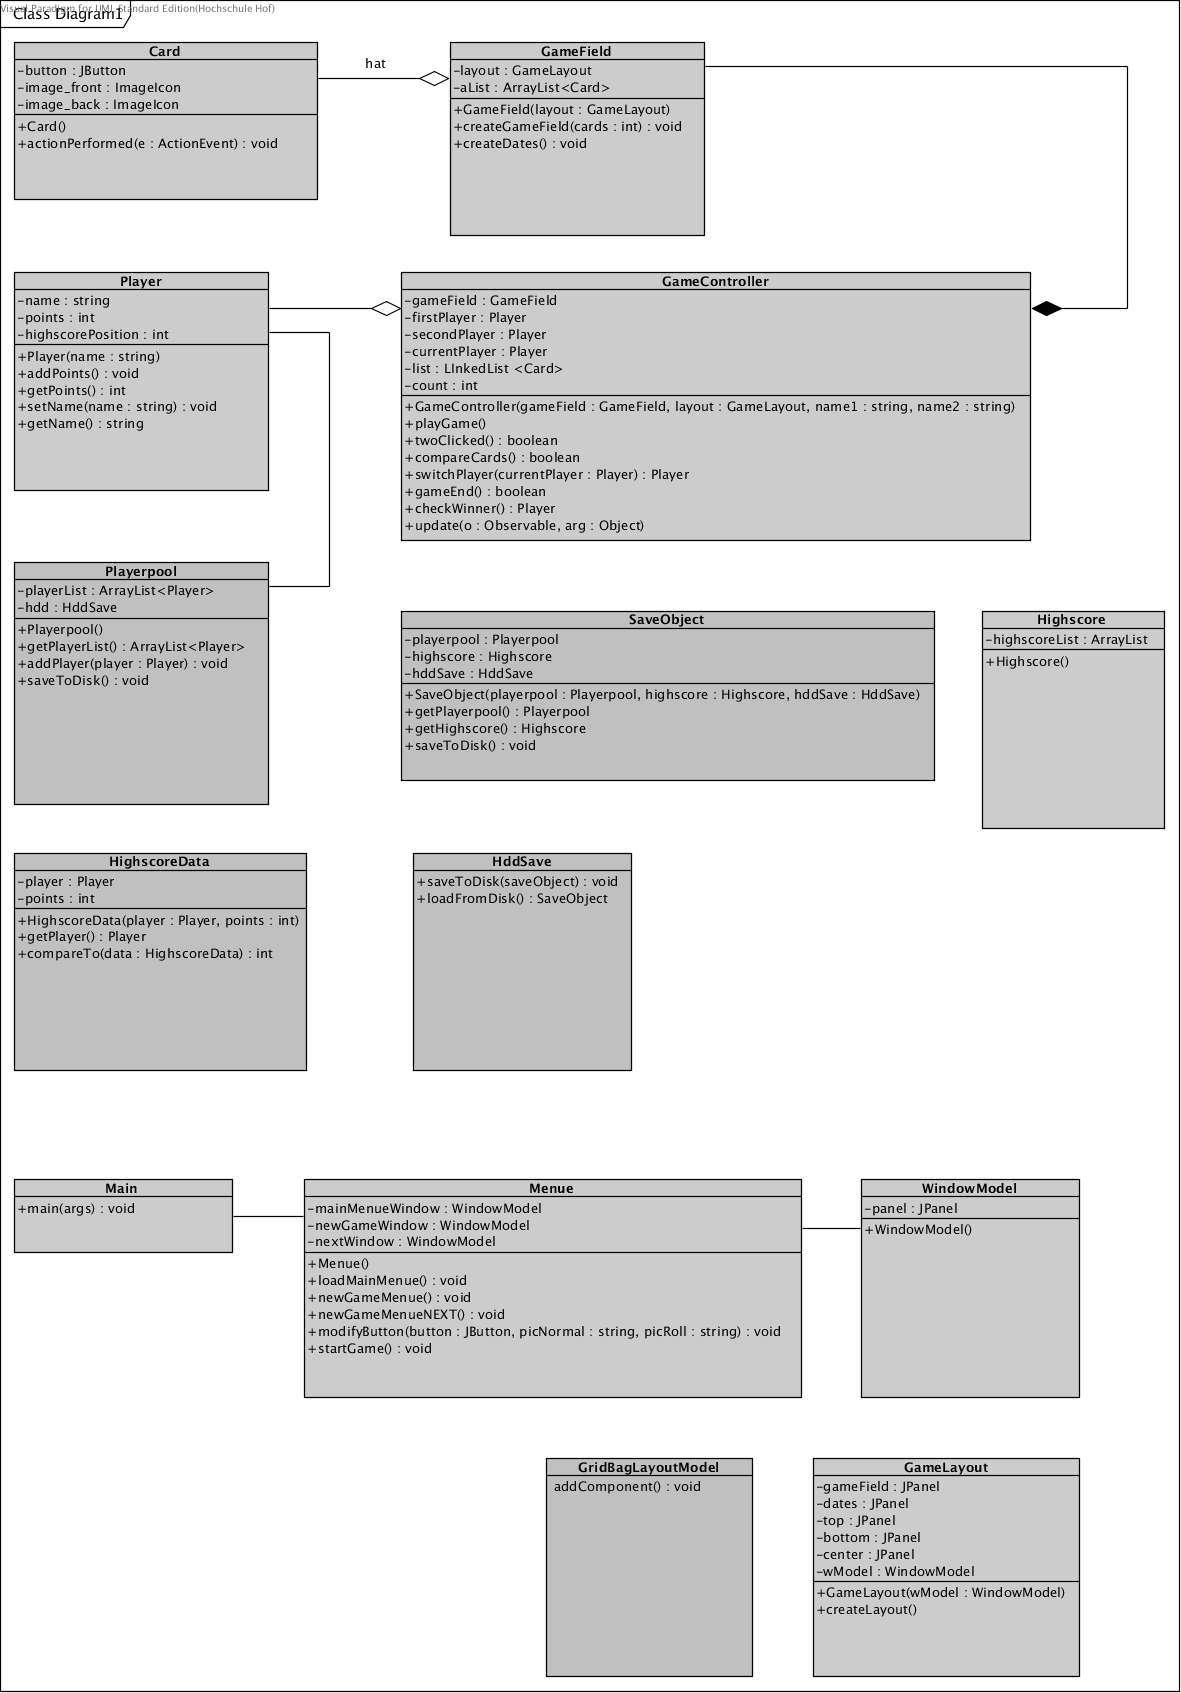
\includegraphics[width=\textwidth]{./Klassendiagramm.png}
	\label{layout_gesamt}
\end{figure}

\begin{figure}[!h]
	\centering
    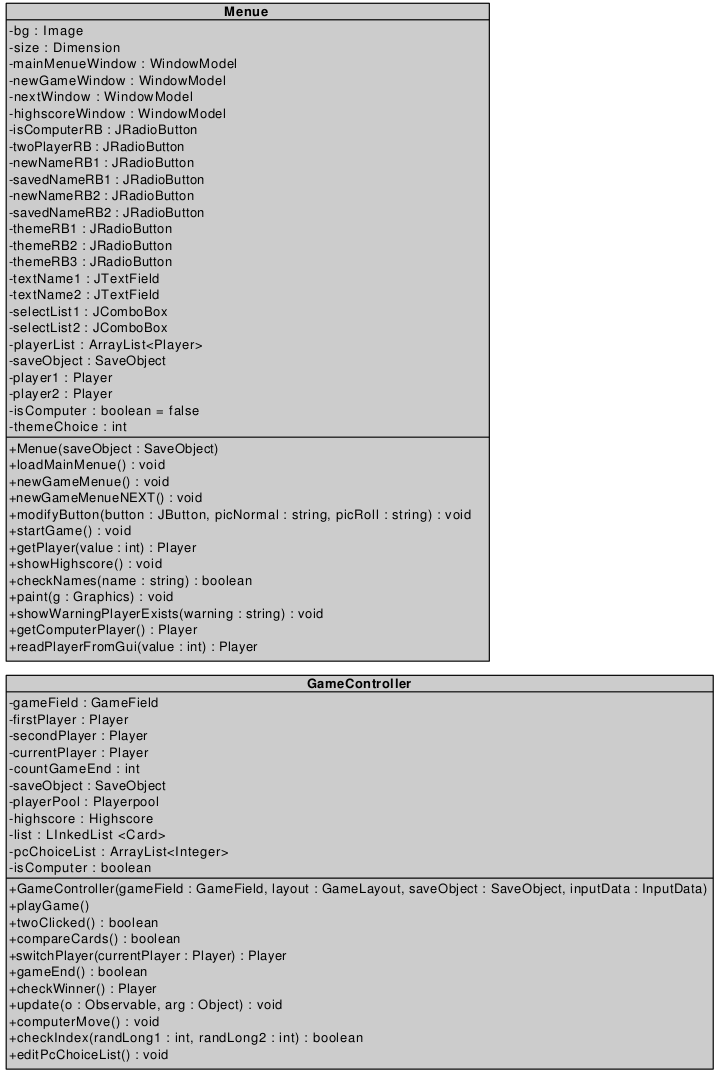
\includegraphics[width=\textwidth]{./Klassendiagramm2.png}
	\label{layout_gesamt}
\end{figure}

\begin{figure}[!t]
	\centering
    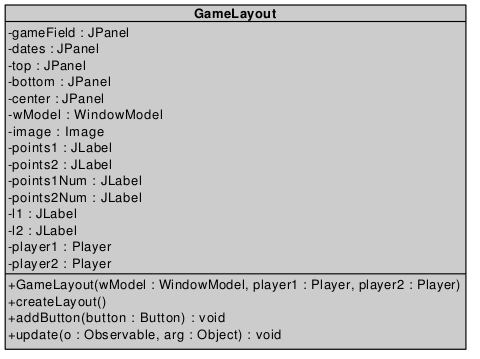
\includegraphics[width=\textwidth]{./Klassendiagramm3.png}
	\label{layout_gesamt}
\end{figure}






